\documentclass[10pt,compress,handout]{beamer}
    \useoutertheme{miniframes}
    \usepackage[english]{babel}
    %\usepackage[margin=1in]{geometry}

    \usepackage{amsmath}
    \usepackage{amsfonts} 
    \usepackage{amssymb}
    \usepackage{amsthm}
    \usepackage{mathtools}

    \usepackage[utf8]{inputenc}
    %\usepackage[exscale, amsfonts, amssymb]{concmath}
    %\renewcommand*{\bfseries}{\mdseries}

    \usepackage{float}
    \usepackage{graphicx}
    \usepackage{caption}
    \usepackage{subcaption}

    \graphicspath{{./src/figures/}}

    %\usepackage{fancyhdr} %custom headers and footers layout
    \usepackage{lastpage} %package to print the last page
    %\pagestyle{fancy} %fancy page style

    \usepackage{textcomp} 
    \usepackage{multicol} 
    \usepackage{multirow}

    \usepackage[table]{xcolor}
    \usepackage{booktabs}

    \usepackage[backend=biber,
    bibstyle=ieee, 
    citestyle=numeric-comp,
    natbib=true,
    doi=false, 
    url=false,
    isbn=false,
    mincitenames=1,
    maxcitenames=1,
    minbibnames=1,
    maxbibnames=99,
    backref=false,]
    {biblatex}
    \addbibresource[label=main]{./src/references.bib}

    \usepackage{url}
    \usepackage{hyperref}

    %edit the properties of your PDF documents which will be displayed
    \hypersetup{
        bookmarks=true, 		% show bookmarks bar?
        unicode=true,  		% non-Latin characters in Acrobat’s bookmarks
        pdftoolbar=true,        % show Acrobat’s toolbar?
        pdfmenubar=true,        % show Acrobat’s menu?
        pdffitwindow=true,      % page fit to window when opened
        pdftitle={PhotoElectrochemistry --- Theoretical Background},    % title
        pdfauthor={M. Skocic},     % author
        pdfsubject={},   % subject of the document
        pdfnewwindow=true,      % links in new window
        pdfkeywords={}, % list of keywords
        colorlinks=false,       % false: boxed links; true: colored links
        linkcolor=red,          % color of internal links
        citecolor=green,        % color of links to bibliography
        filecolor=magenta,      % color of file links
        urlcolor=cyan           % color of external links
    }

    \usepackage{tikz}
    \usepackage{circuitikz}
    \usetikzlibrary{decorations.pathmorphing,arrows,calc}

    \title{PhotoElectroChemistry for Corrosion}
    \author{M. Skocic, PhD Electrochemistry and Materials}
    \date{\vfill 
\includegraphics[width=0.70\textwidth]{full_bw.png}}   

    \setlength{\parskip}{6pt}
    \newcommand{\coef}{1}

\begin{document}
    \begin{frame}
        \titlepage
    \end{frame}

    \begin{frame}
        \frametitle{Contents}
        \tableofcontents
    \end{frame}


% INTRODUCTION
\section{Introduction}
    \begin{frame}{Introduction}
        Photoelectrochemical techniques have been shown to be useful tools for characterizing oxidation layers. 
        
        Interdisciplinary theoretical underpinnings were built \citep{morrison1980, vijh1969, stimming1986, diquarto1997, wouters2007} 
        such as the Gärtner-Butler model \citep{gartner1959,butler1977}
        which has been proven to be a simple and robust model for the photocurrent generation. 
        
        Technical progresses were achieved, allowing to study oxide layers at 
        macroscopic, mesoscopic, and microscopic scales 
        \citep{benaboud2007, srisrual2011}, or in-situ in high temperature corrosion 
        conditions \citep{bojinov2002,skocic2016}.
    \end{frame}

    \begin{frame}{Hypotheses}
        Several hypotheses are needed in order to apply the theoretical concepts:  
        \begin{itemize}
            \item semiconductors are considered to be ideal i.e. crystallized and homogeneous  
            \item the dielectric constant of the semiconductor is independent of the light wavelength  
            \item the capacity of the Helmholtz layer is greater than the capacitance of the space charge capacitance  
            \item the potential drop in the Helmholtz layer is independent of the applied potential and is negligible
        \end{itemize}

        \footnotesize
        \begin{alertblock}{Warning}
            The hypotheses are rarely fully respected in the case of oxides or passive 
            films formed on industrial alloys. Nonetheless, the literature shows that the 
            developed models can be applied to non-ideal systems such as oxides 
            and passive films.
        \end{alertblock}
    \end{frame}



% BASICS
\section{Basics}
\subsection{Electronic Band Structure}
    \begin{frame}[allowframebreaks=1.0]{Band Model}
        Solids: conductors, semiconductors and insulators. 
        
        Valence and conduction bands correspond to allowed energy states for the electrons. 
        
        $E_c$ is the lowest energy level of the conduction band.
        
        $E_v$ is the highest energy level of the valence band.
        
        $E_g$ is the band gap with no allowed energy states. 
        
        $E_F$ is the Fermi level which describes the distribution of the electrons among both bands.
        It represents the highest energy state that can be occupied at 0K. 
        It is equivalent to the electrochemical potential in solid phases.
        
        \framebreak
        The electronic conduction is the movement of electrons and/or holes in conduction/valence band.

        The conduction depends on the number of available charge carriers
        in the conduction band and in the valence band. 
        
        In conductors: overlap of the conduction and the valence bands occurs. 
        
        In semiconductor and insulator: the conduction depends on the band gap and the energy provided by 
        the environment to the electrons from the valence band in order to jump 
        into the conduction band.

        \begin{figure}[h]
            \centering
                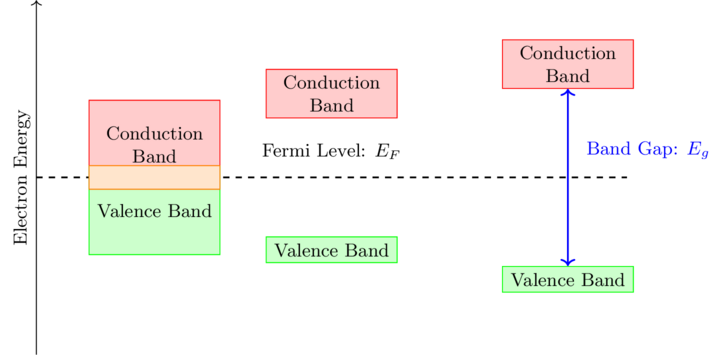
\includegraphics[width=0.5\textwidth]{PEC-band_model.png}
            %\caption{Schematic representation of the electronic band structure \citep{marucco2006}: 
            %a) conductor, b) semiconductor, c) insulator}
            \label{fig_band_model}
        \end{figure}
    \end{frame}

    \begin{frame}{Excitation carrier}
        In semiconductors, charge carriers can be generated by three mechanisms: 
        \begin{itemize}
            \item thermal excitation: in the case of very low band gaps, it can be enough in order 
            to eject an electron from $E_v$ to $E_c$.
            \item photoexcitation: ejects electrons from $E_v$ to $E_c$
            band when an incident photon ($h\nu > E_g$) is absorbed.
            \item doping: introduces additional energy level located in between $E_v$ and $E_c$.
        \end{itemize}
        
        \begin{figure}[h]
            \centering
            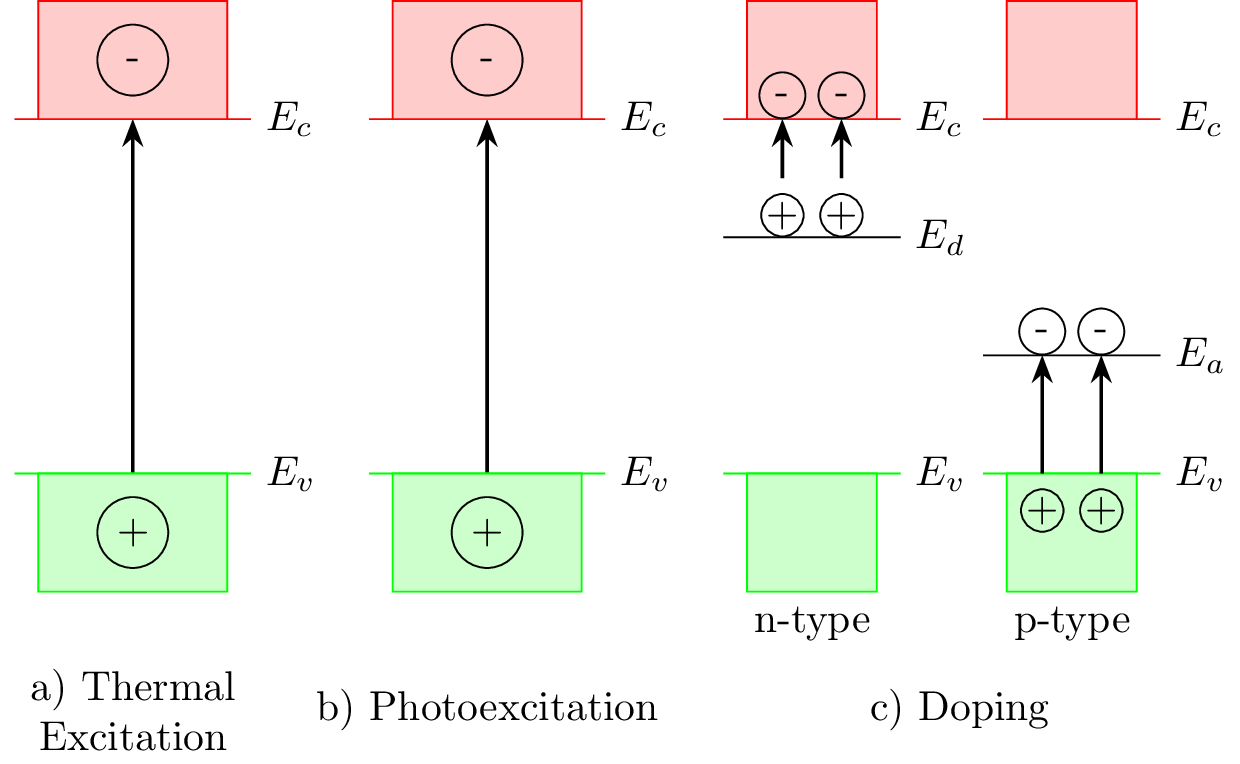
\includegraphics[width=0.5\textwidth]{PEC-excitation_carrier.png}
            %\caption{Schematic representation of the mechanisms generating charge carriers in semiconductors \citep{finklea1983}: 
            %a) thermal excitation, b) photoexcitation, c) doping}
            \label{fig_excitation_carrier}
        \end{figure}
    \end{frame}

    \begin{frame}{Fermi Level Position}
        The Fermi level $E_F$ in intrinsic semiconductors is located at the mid-gap. 
        
        The n-type and p-type doping shift the Fermi level towards band edges 
        $E_c$ and $E_v$.
        
        \begin{figure}[H]
            \centering
            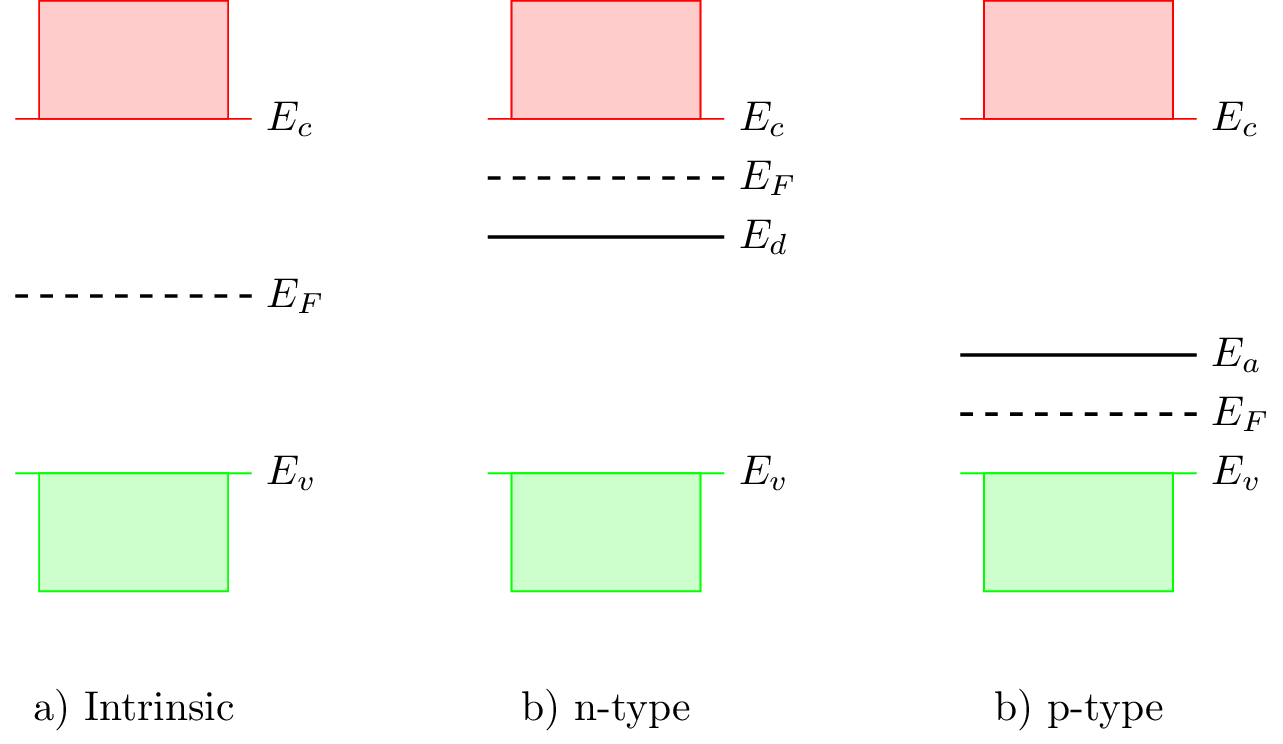
\includegraphics[width=0.5\textwidth]{PEC-fermi_position.png}
            %\caption{Schematic representation of the Fermi level with respect to the 
            %semiconduction type \citep{finklea1983}: a) intrinsic, b) n-type, c) p-type.}
            \label{fig_fermi_position}
        \end{figure}
    \end{frame}

\subsection{Semiconductor/electrolyte interface in dark condition}
    \begin{frame}[allowframebreaks=1.0]{Band Bending}
            A potential gradient occurs when a semiconductor comes into contact with an 
            electrolyte.
            
            $\Phi_{sc}$ and $\Phi_{el}$ correspond to the 
            potentials of the semiconductor and the electrolyte, respectively. 
            
            $\Delta Phi _{sc/el}$ corresponds to the potential difference between 
            the semiconductor and the electrolyte. 
            
            $w_{sc}$ and $w_{H}$ correspond to 
            the widths of the space charge and the electrical double layer, 
            respectively.

        \begin{figure}[h]
            \centering
            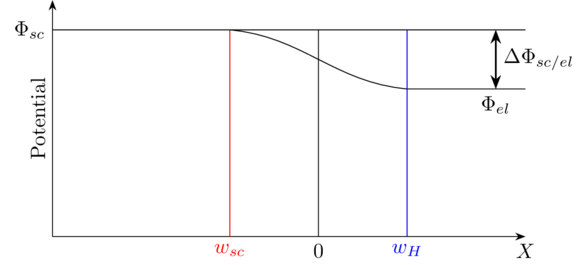
\includegraphics[width=0.5\textwidth]{PEC-interface_potential.png}
            %\caption{Potential gradient at semiconductor/electrolyte interface 
            %\citep{marcus2006}. $\Phi_{sc}$ and $\Phi_{el}$ correspond to the 
            %potentials of the semiconductor and the electrolyte, respectively. 
            %$\Delta Phi _{sc/el}$ corresponds to the potential difference between 
            %the semiconductor and the electrolyte. $w_{sc}$ and $w_{H}$ correspond to 
            %the widths of the space charge and the electrical double layer, 
            %respectively.}
            \label{fig_interface_potential}
        \end{figure}

        \framebreak
            
        The position of the Fermi level in the electrolyte with respect to the 
        conduction and valence band edges leads to three different situations after 
         a transient charge transfer:
        \begin{itemize}
            \item flat band
            \item depletion
            \item accumulation
        \end{itemize}
        
        The flat band situation occurs when the Fermi level in the electrolyte 
        matches the Fermi level in the semiconductor. 
        
        Consequently, there is no potential gradient in the semiconductor. 
        
        In a case of Fermi level mismatch, a band bending occurs in the semiconductor 
        near the semiconductor/electrolyte interface.  
        
        \framebreak
        The band bending leads to either depletion or accumulation of majority 
        charge carriers near the semiconductor/electrolyte interface. 
        
        The spatial extension of the depletion/accumulation zone is called space 
        charge.
    
        \begin{figure}[H]
            \centering
            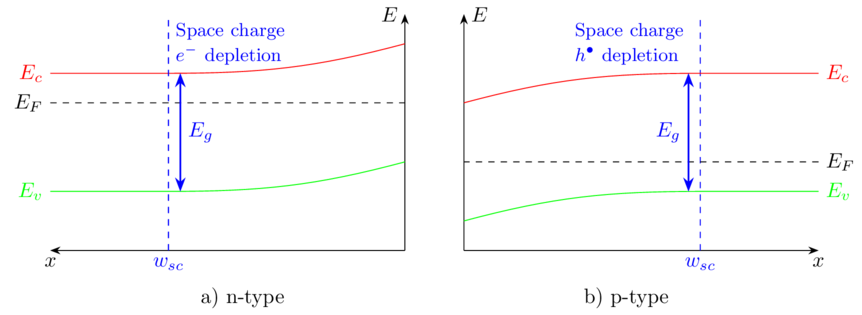
\includegraphics[width=0.85\textwidth]{PEC-space_charge_depletion.png}
            %\caption{Schematic representation of the space charge in depletion of majority charge carriers for 
            %a semiconductor in contact with an electrolyte \citep{memming2008,bard2002}:
            % a) n-type, b) p-type.}
            \label{fig_space_charge_depletion}
        \end{figure}

        \framebreak
        
        Depletion and accumulation as well as band bending can be obtained 
        by polarizing the semiconductor.
        
        Depending on the applied potential, $U$, with respect to the flat band 
        potential, $U_{fb}$, three different situations will occur:
        \begin{itemize}
            \item $U = U_{fb}$: flat band situation no matter the semiconductor type
            \item $U > U_{fb}$: depletion (accumulation) in a case of n-type (p-type) semiconductor  
            \item $U < U_{fb}$: accumulation (depletion) in a case of n-type (p-type) semiconductor
        \end{itemize}
        
        \begin{figure}[H]
        \centering
            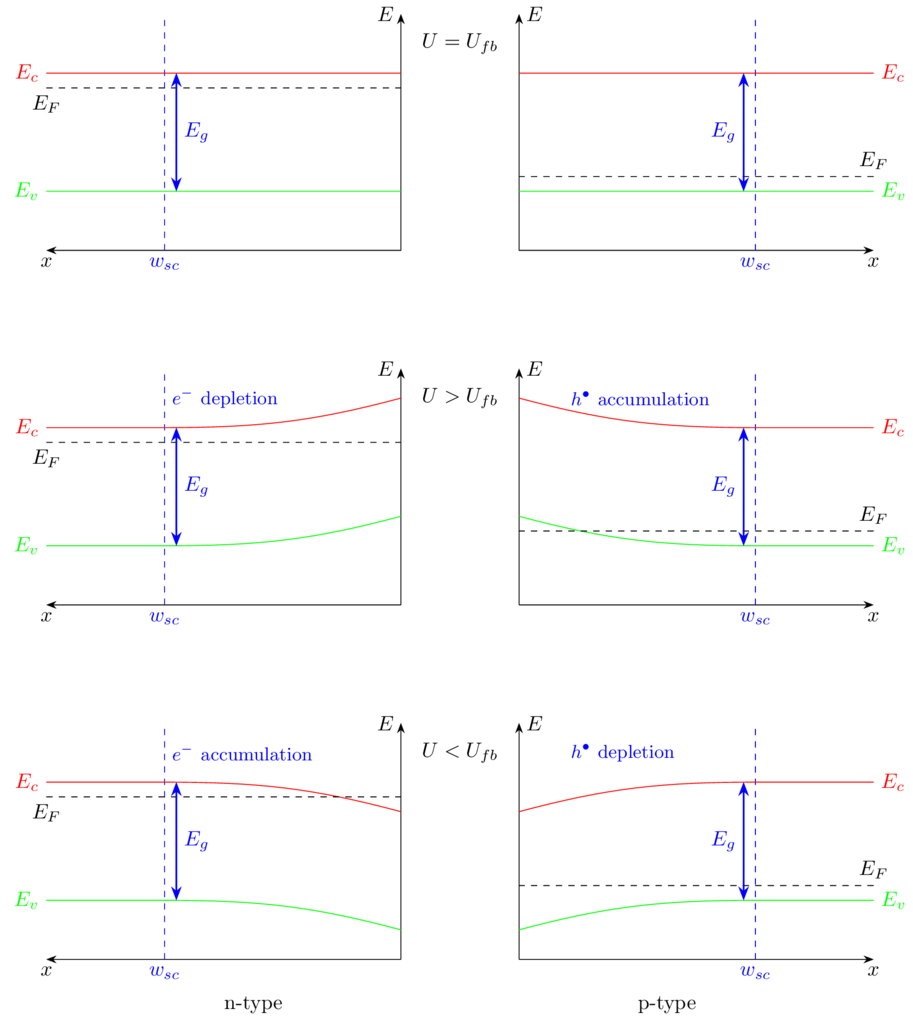
\includegraphics[width=0.6\textwidth]{PEC-band_bending.png}
            %\caption{Schematic representation of the band bending in p-type and n-type 
            %semiconductors in contact with an electrolyte \citep{memming2008, bard2002}:
            % a) $U = U_{fb}$, b) $U > U_{fb}$, c) $U < U_{fb}$.}
            \label{fig_band_bending}
        \end{figure}
    
        Without illumination, cathodic (anodic) currents are favored in a case of 
        accumulation of electrons (holes) for an n-type (p-type) semiconductor. 
        
        In fact, the majority charge carriers of n-type (p-type) semiconductors are 
        electrons (holes). 
        
        Reciprocally, anodic (cathodic) currents are not favored in a case of 
        depletion of electrons (holes) for an n-type (p-type) semiconductor. 
        
        The junction between a semiconductor and an electrolyte acts like a Schottky diode.
    \end{frame}

\subsection{Semiconductor/electrolyte interface under illumination}
    \begin{frame}[allowframebreaks=1.0]{Electron/hole pairs}
        The illumination of the semiconductor/electrolyte interface, 
        with photons having an energy greater than the band gap, $E_g$, creates 
        electron/hole pairs in the semiconductor. 
        
        By applying the adequate potential the pairs can be separated. 
        
        As a consequence, the majority charge carriers are attracted to the 
        semiconductor bulk whereas the minority charge carriers are drawn to the 
        semiconductor/electrolyte interface where they can be transferred to a RedOx 
        species creating an additional current called photocurrent. 
    
        \begin{figure}[h]
            \centering
            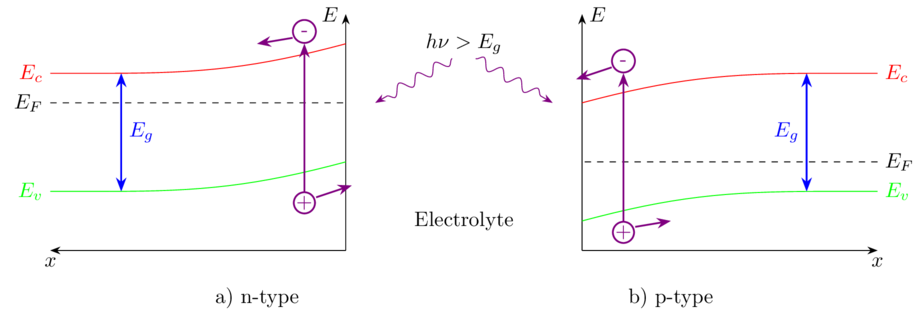
\includegraphics[width=0.65\textwidth]{PEC-photocurrent_generation.png}
            %\caption{Schematic representation of the mechanism generating 
            %a photocurrent \citep{memming2008,bard2002}.}
            \label{fig_photocurrent_generation}
        \end{figure}
    
        The photocurrent is significant when the semiconductor/electrolyte junction 
        is in depletion. 
        
        n-type (p-type) 
        semiconductors generate anodic (cathodic) photocurrents where the 
        electrons (holes) move towards the external circuit whereas the holes (electrons) 
        move towards the interface. 
        
        The applied potential on n-type (p-type) semiconductors is 
        greater (lower) than the flat band potential. \index{potential!flat band}

        \begin{figure}[h]
            \centering
            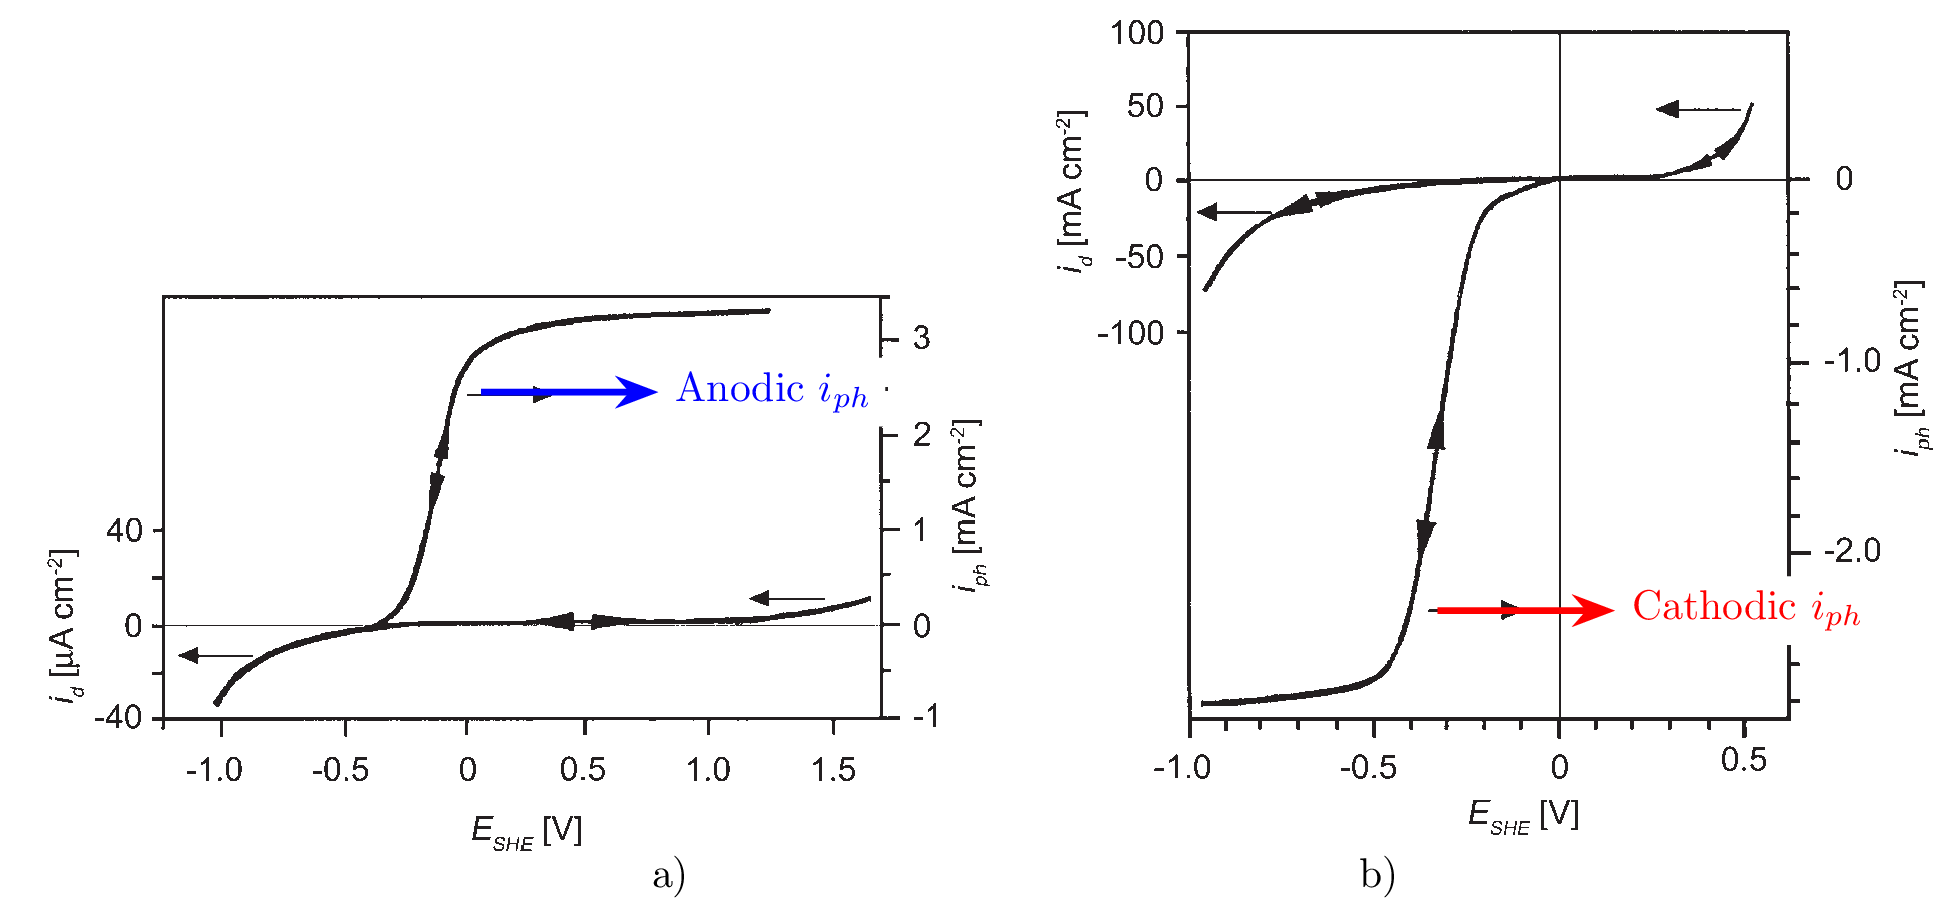
\includegraphics[width=0.65\textwidth]{PEC-photocurrent_plieth.png}
            %\caption{Photocurrent density $i_{ph}$ and dark current density 
            %$i_d$ with respect to the potential in a case of GaAs semiconductor 
            %\citep{plieth2008}: a) n-type, b) p-type.}
            \label{fig_photocurrent_plieth}
        \end{figure}

    \end{frame}


    \begin{frame}[allowframebreaks=1.0]{Gärtner-Butler Model}
        \citet{gartner1959} and \citet{butler1977} proposed a simple and robust model for 
        describing the photocurrent.
        
        The photocurrent depends on:  
            \begin{itemize}
                \item $w_{sc}$: space charge width 
                \item $\alpha$: absorption coefficient
                \item $L_{cc }$: the average diffusion length of the minority charge carriers
            \end{itemize}

        \begin{equation}
            I_{ph} = \phi _0 \left[ 1 - \frac{\exp (-\alpha _{sc} \cdot w_{sc})}{1+\alpha _{sc} \cdot
            L_{cc}} \right]
            \label{eq_iph_gartner_butler}
        \end{equation}
        
        When $\alpha _{sc} \cdot w_{sc} \ll 1$ and $\alpha _{\sc} \cdot L_{cc} \ll 1$, 
        the photocurrent is approximated by the 
        equation~\ref{eq_iph_gartner_butler_simplified}.

        \begin{equation}
            I_{ph} = \phi _0 \cdot \alpha _{\sc} \cdot w_{sc}
            \label{eq_iph_gartner_butler_simplified}
        \end{equation}
        
        %\footnotesize
        %\begin{alertblock}{Warning}
        %    All absorbed photons generate electron/hole pairs and 
        %    the minority charge carriers are transferred to the electrolyte and 
        %    therefore contribute to the photocurrent.
        %\end{alertblock}

        \framebreak
        Space charge width $w_{sc}$ in depletion depends on:
        \begin{itemize}
            \item $N_{cc}$: number of majority charge carriers ($\sim$ doping) 
            \item $e$: elementary charge of an electron 
            \item $U$, $U_{fb}$: applied, flat band potentials
            \item $\epsilon$, $\epsilon _0$: relative, vacuum permittivity
        \end{itemize}

        \begin{equation}
            w_{sc} = \sqrt{ \frac{2\epsilon \epsilon _0}{e N_{cc}} (U-U_{fb}-\frac{kT}{e}) }
            \label{eq_space_charge_Schottky}
        \end{equation}
        
        The absorption coefficient $\alpha _{sc}$ depends on $h\nu$ (light energy) and $n$ (band-band transition type).

        \begin{equation}
            \alpha _{sc} = const \frac{(h\nu - E_g)^n}{h\nu}
            \label{eq_absorption_coef}
        \end{equation}

        \framebreak
        The photocurrent is therefore given by the 
        equation~\ref{eq_iph_substitute_W_alpha}. 

        \begin{equation}
            I_{ph} = \phi _0 \cdot const \frac{(h\nu - E_g)^n}{h\nu}
                \cdot \sqrt{ \frac{2\epsilon \epsilon _0}{e N_{cc}} (U-U_{fb}-\frac{kT}{e}) }
            \label{eq_iph_substitute_W_alpha}
        \end{equation}
        
        The linear transform with respect to the energy is used for determining the band gaps. 
        \begin{equation}
            \left[ \frac{I_{ph} \cdot h\nu}{\phi _0} \right] ^{1/n} = const \cdot (h\nu - E_g)
            \label{eq_iph_linear_transform}
        \end{equation}
        
        The linear transform with respect to the potential  is used for determining 
        the semiconducting type, the flat band potential, 
        and the number of majority charge carrier.
        \begin{equation}
            I_{ph}^2 = const \cdot (U-U_{fb}-\frac{kT}{e})
            \label{eq_iph_linear_transform_potential}
        \end{equation}
    \end{frame}



% APPLICATIONS 
\section{Applications}
\subsection{Minor oxides}
    \begin{frame}{Identification of minor oxides}
        \citet{benaboud2007} showed that the photoelectrochemical characterization 
        is robust for detecting the presence of minor oxides. 
        
        The strong photocurrent observed at around 5~eV 
        reveals the major oxide i.e. monoclinic zirconia. 
        The photocurrent $h\nu < 5 eV$ reveals the presence of minor 
        oxides even in “pure” zirconium. 
        
        The slope changes provided an estimation of the band gaps: 
        hematite, chromia and a solid solution of $(Fe_xCr_{1-x})O_3$. 

        \renewcommand{\coef}{0.45}
        \begin{figure}[h]
            \centering
            \begin{subfigure}{\coef\textwidth}
                \centering
                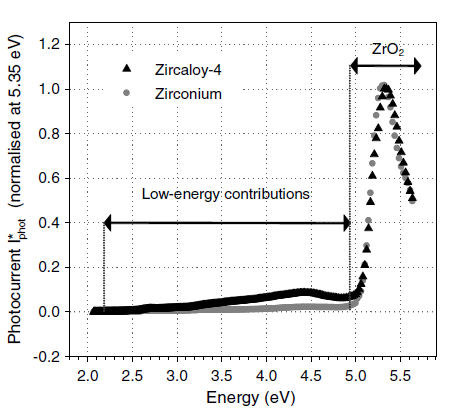
\includegraphics[width=0.65\textwidth]{./src/figures/Benaboud2007-Fig4.png}
                \caption{}
                \label{fig_benaboud_minor_oxides_a}
            \end{subfigure}
            \begin{subfigure}{\coef\textwidth}
                \centering
                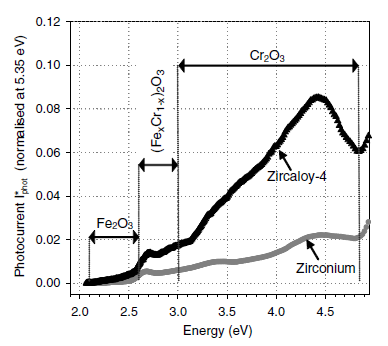
\includegraphics[width=0.65\textwidth]{./src/figures/Benaboud2007-Fig5.png}
                \caption{}
                \label{fig_benaboud_minor_oxides_b}
            \end{subfigure}
            
            %\caption{Photocurrent spectra measured on zirconia oxide layer formed on 
            %Zircaloy4 and “pure” zirconium oxidized for 1h at 470°C in oxygenated 
            %atmosphere\citep{benaboud2007}: a) complete spectrum b) close-up view on the minor contributions.}
            \label{fig_benaboud_minor_oxides}
        \end{figure}
    \end{frame}

\subsection{Semiconducting type}
    \begin{frame}{Semiconduction type}
            \citet{loucif2013} showed the effect of hydrogen pressure on 
            the semiconduction type on Ni-based alloy 600 oxidized in simulated PWR. 
            
            The “V-shape” of the normalized photocurrent 
            reveals an isolating behavior of the oxide layer at high hydrogen pressure. 
            
            The monotonous increase of the 
            normalized photocurrent towards more anodic potentials reveals 
            n-type semiconduction.

        \renewcommand{\coef}{0.45}
        \begin{figure}[h]
            \centering
            \begin{subfigure}{\coef\textwidth}
                \centering
                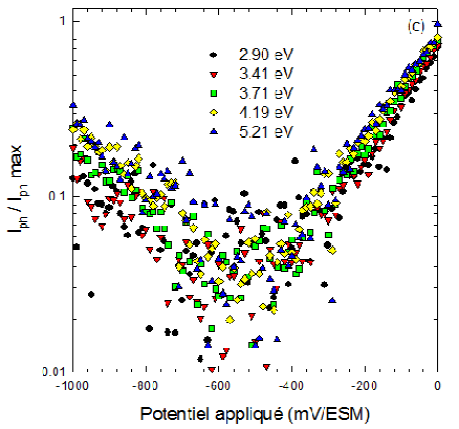
\includegraphics[width=0.65\textwidth]{./src/figures/Loucif2012-Fig3-18.png}
                \caption{}
                \label{fig_loucif_sctype_a}
            \end{subfigure}
            \begin{subfigure}{\coef\textwidth}
                \centering
                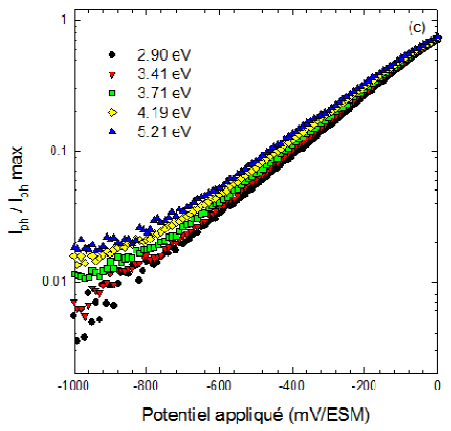
\includegraphics[width=0.65\textwidth]{./src/figures/Loucif2012-Fig3-19.png}
                \caption{}
                \label{fig_loucif_sctype_b}
            \end{subfigure}
            
            %\caption{Photocurrent with respect to the potential for an 
            %Ni-based alloy 600 polished and oxidized in simulated PWR 
            %for 500~h \citep{loucif2013}: a) $P_{H_2}$=6.5~bar, b) $P_{H_2}$=0.05~bar.}
            \label{fig_loucif_sctype}
        \end{figure}
    \end{frame}

\subsection{High temperature PEC}
    \begin{frame}[allowframebreaks=1.0]{High temperature PEC}
        The majority of photoelectrochemical characterizations are performed at 
        room temperature in simple glass/Plexiglas cells where the signal/noise 
        ratio is very good.
        
        High temperature photoelectrochemical characterizations 
        require sophisticated metallic cells and transparent windows 
        able to withstand the arch environment. 
        
        Despite the need to improve the signal/noise ratio, the feasibility of 
        the in-situ photoelectrochemical characterizations was demonstrated by 
        \citet{bojinov2002} in 2002 and more recently by \citet{skocic2016} in 2015 

        \renewcommand{\coef}{0.45}
        \begin{figure}[h]
            \centering
            \begin{subfigure}{\coef\textwidth}
                \centering
                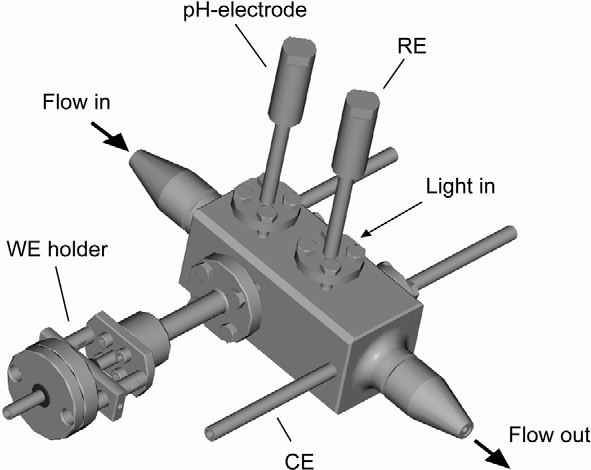
\includegraphics[width=\textwidth]{./src/figures/Bojinov_2002_Fig1.png}
                \caption{}
                \label{fig_bojinov_ht_a}
            \end{subfigure}
            \begin{subfigure}{\coef\textwidth}
                \centering
                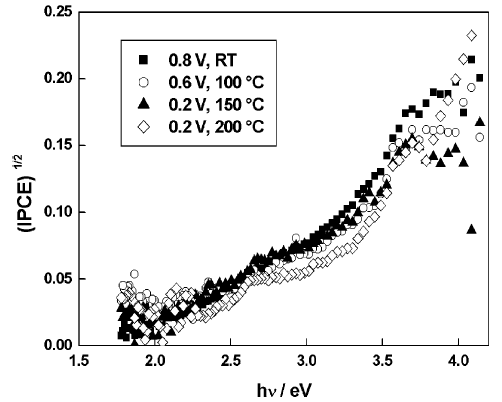
\includegraphics[width=\textwidth]{./src/figures/Bojinov_2002_Fig5b.png}
                \caption{}
                \label{fig_bojinov_ht_b}
            \end{subfigure}
            
            %\caption{a) Schematic representation of the metallic cell developed
            %by \citet{bojinov2002}. 
            %b) Photocurrent spectra performed on iron oxides at different 
            %temperatures (up to 200°C) obtained by \citet{bojinov2002}.}
            \label{fig_bojinov_ht}
        \end{figure}

        \renewcommand{\coef}{0.45}
        \begin{figure}[h]
            \centering
            \begin{subfigure}{\coef\textwidth}
                \centering
                \includegraphics[width=\textwidth]{./src/figures/skocic2015-1.png}
                \caption{}
                \label{fig_skocic_phd_cell}
            \end{subfigure}
            \begin{subfigure}{\coef\textwidth}
                \centering
                \includegraphics[width=\textwidth]{./src/figures/skocic2015-2.png}
                \caption{}
                \label{fig_skocic_phd_htpec}
            \end{subfigure}
            
            %\caption{a) Schematic view of the photoelectrochemical cell developed by \citet{skocic2016}. 
            %b) Photocurrent energy spectra of an X750 specimen recorded at room
            %temperature and in 280°C/80 bar water \citep{skocic2016}}
            \label{fig_skocic_phd}
        \end{figure}
    \end{frame}




% BIBLIOGRAPHY
\begin{frame}[allowframebreaks=0.9]{References}
\AtNextBibliography{\tiny}
%\nocite{*}
\printbibliography
\end{frame}

\end{document}
